% 第十五章：勒让德函数

\chapter{勒让德函数}

\begin{wulibj}[本章导读]
勒让德函数是求解球对称问题中拉普拉斯方程时自然出现的特殊函数。本章我们将学习勒让德多项式\index{勒让德多项式}的定义、性质及其应用，为求解球坐标系下的数学物理问题奠定基础。
\end{wulibj}

% ========== 第一节 ==========
\section{勒让德方程的导出}

\subsection{球坐标系下拉普拉斯方程的分离变量}

在球坐标系 $(r, \theta, \varphi)$ 中，拉普拉斯方程为
\begin{equation}
    \frac{1}{r^2}\frac{\partial}{\partial r}\left(r^2\frac{\partial u}{\partial r}\right) + \frac{1}{r^2\sin\theta}\frac{\partial}{\partial\theta}\left(\sin\theta\frac{\partial u}{\partial\theta}\right) + \frac{1}{r^2\sin^2\theta}\frac{\partial^2 u}{\partial\varphi^2} = 0
\end{equation}

设 $u(r, \theta, \varphi) = R(r)Y(\theta, \varphi)$，分离变量得：
\begin{equation}
    \frac{1}{R}\frac{\mathrm{d}}{\mathrm{d}r}\left(r^2\frac{\mathrm{d}R}{\mathrm{d}r}\right) = -\frac{1}{Y}\left[\frac{1}{\sin\theta}\frac{\partial}{\partial\theta}\left(\sin\theta\frac{\partial Y}{\partial\theta}\right) + \frac{1}{\sin^2\theta}\frac{\partial^2 Y}{\partial\varphi^2}\right] = \lambda
\end{equation}

\subsection{轴对称情形}

对于轴对称问题（与 $\varphi$ 无关），设 $Y(\theta) = \Theta(\theta)$，得
\begin{equation}
    \frac{1}{\sin\theta}\frac{\mathrm{d}}{\mathrm{d}\theta}\left(\sin\theta\frac{\mathrm{d}\Theta}{\mathrm{d}\theta}\right) + \lambda\Theta = 0
\end{equation}

令 $x = \cos\theta$，$\Theta(\theta) = y(x)$，方程变为
\begin{equation}
    \boxed{(1-x^2)\frac{\mathrm{d}^2 y}{\mathrm{d}x^2} - 2x\frac{\mathrm{d}y}{\mathrm{d}x} + \lambda y = 0}
\end{equation}

这就是\textbf{勒让德方程}。

要求解在 $x = \pm 1$（$\theta = 0, \pi$）处有限，需要 $\lambda = l(l+1)$，$l = 0, 1, 2, \ldots$。

% ========== 第二节 ==========
\section{勒让德多项式\index{勒让德多项式}}

\subsection{幂级数解法}

设勒让德方程的解为幂级数 $y(x) = \sum_{k=0}^{\infty} a_k x^k$。

代入方程，得到递推关系：
\begin{equation}
    a_{k+2} = \frac{k(k+1) - \lambda}{(k+1)(k+2)}a_k
\end{equation}

当 $\lambda = l(l+1)$ 时，级数在某项截断，成为多项式。

\subsection{勒让德多项式\index{勒让德多项式}的定义}

\begin{zhongyao}[勒让德多项式的罗德里格斯公式]
\[
    P_l(x) = \frac{1}{2^l l!}\frac{\mathrm{d}^l}{\mathrm{d}x^l}(x^2 - 1)^l
\]
\end{zhongyao}

前几个勒让德多项式\index{勒让德多项式}：
\begin{align}
    P_0(x) &= 1 \\
    P_1(x) &= x \\
    P_2(x) &= \frac{1}{2}(3x^2 - 1) \\
    P_3(x) &= \frac{1}{2}(5x^3 - 3x) \\
    P_4(x) &= \frac{1}{8}(35x^4 - 30x^2 + 3)
\end{align}

\begin{figure}[htbp]
\centering
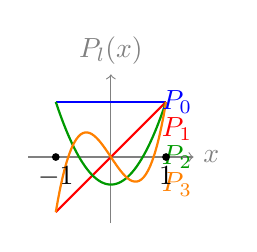
\begin{tikzpicture}[scale=0.7]
    \draw[->, gray] (-1.5, 0) -- (1.5, 0) node[right] {$x$};
    \draw[->, gray] (0, -1.2) -- (0, 1.5) node[above] {$P_l(x)$};
    
    \draw[blue, thick, domain=-1:1, samples=50] plot (\x, {1});
    \draw[red, thick, domain=-1:1, samples=50] plot (\x, {\x});
    \draw[green!60!black, thick, domain=-1:1, samples=50] plot (\x, {0.5*(3*\x*\x - 1)});
    \draw[orange, thick, domain=-1:1, samples=50] plot (\x, {0.5*(5*\x*\x*\x - 3*\x)});
    
    \node[blue] at (1.2, 1) {$P_0$};
    \node[red] at (1.2, 0.5) {$P_1$};
    \node[green!60!black] at (1.2, 0) {$P_2$};
    \node[orange] at (1.2, -0.5) {$P_3$};
    
    \fill (-1, 0) circle (2pt);
    \fill (1, 0) circle (2pt);
    \node[below] at (-1, 0) {$-1$};
    \node[below] at (1, 0) {$1$};
\end{tikzpicture}
\caption{勒让德多项式\index{勒让德多项式}}
\label{fig:legendre-polynomials}
\end{figure}

\subsection{勒让德多项式\index{勒让德多项式}的性质}

\begin{dingli}{}{奇偶性}
\begin{equation}
    P_l(-x) = (-1)^l P_l(x)
\end{equation}
即 $P_l(x)$ 当 $l$ 为偶数时是偶函数，$l$ 为奇数时是奇函数。
\end{dingli}

\begin{proof}
由罗德里格斯公式：
\begin{equation}
    P_l(x) = \frac{1}{2^l l!}\frac{\mathrm{d}^l}{\mathrm{d}x^l}(x^2 - 1)^l
\end{equation}
设 $x \to -x$，则 $(x^2 - 1)^l$ 不变，但每求一次导数多一个负号。求 $l$ 次导数后，得
\begin{equation}
    P_l(-x) = (-1)^l P_l(x)
\end{equation}
\end{proof}
\begin{dingli}{}{特殊值}
\begin{equation}
    P_l(1) = 1, \quad P_l(-1) = (-1)^l
\end{equation}
\end{dingli}

\begin{proof}
在母函数中取 $x = 1$：
\begin{equation}
    \frac{1}{1 - t} = \sum_{l=0}^{\infty} P_l(1) t^l
\end{equation}
左边泰勒展开为 $\sum_{l=0}^{\infty} t^l$，比较系数得 $P_l(1) = 1$。

由奇偶性，$P_l(-1) = (-1)^l P_l(1) = (-1)^l$。
\end{proof}
\begin{dingli}{}{递推公式}
\begin{equation}
    \boxed{(l+1)P_{l+1}(x) = (2l+1)xP_l(x) - lP_{l-1}(x)}
\end{equation}
\end{dingli}

\begin{proof}
由母函数 $G(x,t) = \frac{1}{\sqrt{1-2xt+t^2}}$，对 $t$ 求偏导：
\begin{equation}
    \frac{\partial G}{\partial t} = \frac{x - t}{(1 - 2xt + t^2)^{3/2}} = \frac{x - t}{1 - 2xt + t^2} G
\end{equation}
将 $G = \sum_{l=0}^{\infty} P_l(x)t^l$ 代入，得
\begin{equation}
    \sum_{l=0}^{\infty} lP_l(x)t^{l-1} = \frac{x - t}{1 - 2xt + t^2} \sum_{l=0}^{\infty} P_l(x)t^l
\end{equation}
交叉相乘并比较 $t^l$ 的系数，即得递推公式。
\end{proof}
\begin{dingli}{}{母函数}
\begin{equation}
    \boxed{\frac{1}{\sqrt{1 - 2xt + t^2}} = \sum_{l=0}^{\infty} P_l(x)t^l, \quad |t| < 1}
\end{equation}
\end{dingli}

\begin{proof}
设 $f(x, t) = (1 - 2xt + t^2)^{-1/2}$，验证 $P_l(x)$ 由罗德里格斯公式给出时满足此展开。

方法一：设 $f(x, t) = \sum_{l=0}^{\infty} a_l(x) t^l$，由勒让德方程可证 $a_l(x)$ 满足勒让德方程，且归一化条件 $a_l(1) = 1$ 确定常数。

方法二：直接验证罗德里格斯公式的泰勒展开。由二项式展开：
\begin{equation}
    (1 - 2xt + t^2)^{-1/2} = \sum_{k=0}^{\infty} \binom{-1/2}{k} (-2xt + t^2)^k
\end{equation}
展开并整理 $t^l$ 的系数，可得 $P_l(x)$ 的表达式。
\end{proof}
\begin{wulibj}[母函数的物理意义]
母函数是单位电荷在距离 $1/t$ 处产生的电势展开式。这给出了勒让德多项式\index{勒让德多项式}的物理来源。
\end{wulibj}

\subsection{正交性}

\begin{zhongyao}[勒让德多项式的正交性]
勒让德多项式在 $[-1, 1]$ 上正交：
\[
    \int_{-1}^{1} P_m(x)P_n(x)\,\mathrm{d}x = \frac{2}{2n+1}\delta_{mn}
\]
\end{zhongyao}

\begin{proof}
设 $m < n$，$P_m(x)$ 是 $m$ 次多项式，$P_n(x)$ 是 $n$ 次多项式。

由勒让德方程：
\begin{equation}
    \frac{\mathrm{d}}{\mathrm{d}x}\left[(1-x^2)P_m'(x)\right] + m(m+1)P_m(x) = 0
\end{equation}

乘以 $P_n(x)$ 并积分：
\begin{equation}
    \int_{-1}^{1} P_n(x)\frac{\mathrm{d}}{\mathrm{d}x}\left[(1-x^2)P_m'(x)\right]\,\mathrm{d}x + m(m+1)\int_{-1}^{1} P_m(x)P_n(x)\,\mathrm{d}x = 0
\end{equation}

分部积分第一项：
\begin{equation}
    \left[(1-x^2)P_m'(x)P_n(x)\right]_{-1}^{1} - \int_{-1}^{1} (1-x^2)P_m'(x)P_n'(x)\,\mathrm{d}x = -\int_{-1}^{1} (1-x^2)P_m'(x)P_n'(x)\,\mathrm{d}x
\end{equation}

同理，交换 $m$ 和 $n$，两式相减得：
\begin{equation}
    [n(n+1) - m(m+1)]\int_{-1}^{1} P_m(x)P_n(x)\,\mathrm{d}x = 0
\end{equation}

当 $m \neq n$ 时，积分等于零。
\end{proof}

\subsection{广义傅里叶级数}

任何在 $[-1, 1]$ 上分段光滑的函数 $f(x)$ 可以展开为勒让德多项式\index{勒让德多项式}级数：
\begin{equation}
    f(x) = \sum_{l=0}^{\infty} c_l P_l(x)
\end{equation}

其中
\begin{equation}
    \boxed{c_l = \frac{2l+1}{2}\int_{-1}^{1} f(x)P_l(x)\,\mathrm{d}x}
\end{equation}

% ========== 第三节 ==========
\section{连带勒让德函数}

\subsection{连带勒让德方程}

当问题不具有轴对称性时，$\varphi$ 方向分离出 $m^2$：
\begin{equation}
    (1-x^2)\frac{\mathrm{d}^2 y}{\mathrm{d}x^2} - 2x\frac{\mathrm{d}y}{\mathrm{d}x} + \left[l(l+1) - \frac{m^2}{1-x^2}\right]y = 0
\end{equation}

这是\textbf{连带勒让德方程}。

\subsection{连带勒让德函数的定义}

\begin{dingliyi}{}{连带勒让德函数}
连带勒让德方程的解称为连带勒让德函数：
\begin{equation}
    \boxed{P_l^m(x) = (1-x^2)^{m/2}\frac{\mathrm{d}^m}{\mathrm{d}x^m}P_l(x), \quad m = 0, 1, \ldots, l}
\end{equation}
\end{dingliyi}

\begin{tishi}
$P_l^0(x) = P_l(x)$，勒让德多项式\index{勒让德多项式}是连带勒让德函数的特例。
\end{tishi}

正交性：
\begin{equation}
    \int_{-1}^{1} P_l^m(x)P_{l'}^m(x)\,\mathrm{d}x = \frac{2}{2l+1}\frac{(l+m)!}{(l-m)!}\delta_{ll'}
\end{equation}

% ========== 第四节 ==========
\section{球谐函数}

\subsection{定义}

\begin{dingliyi}{}{球谐函数}
球谐函数定义为
\begin{equation}
    \boxed{Y_l^m(\theta, \varphi) = \sqrt{\frac{2l+1}{4\pi}\frac{(l-m)!}{(l+m)!}}P_l^m(\cos\theta)\mathrm{e}^{im\varphi}}
\end{equation}
其中 $l = 0, 1, 2, \ldots$，$m = -l, -l+1, \ldots, l$。
\end{dingliyi}

\subsection{性质}

\begin{dingli}{}{正交归一性}
\begin{equation}
    \int_0^{2\pi}\int_0^{\pi} Y_l^m(\theta, \varphi)Y_{l'}^{m'*}(\theta, \varphi)\sin\theta\,\mathrm{d}\theta\,\mathrm{d}\varphi = \delta_{ll'}\delta_{mm'}
\end{equation}
\end{dingli}

\begin{proof}
由球谐函数的定义，积分分为两部分：
\begin{equation}
    \int_0^{2\pi}\int_0^{\pi} Y_l^m Y_{l'}^{m'*} \sin\theta\,\mathrm{d}\theta\,\mathrm{d}\varphi = C \int_0^{\pi} P_l^m(\cos\theta)P_{l'}^{m'}(\cos\theta)\sin\theta\,\mathrm{d}\theta \cdot \int_0^{2\pi} \mathrm{e}^{i(m-m')\varphi}\,\mathrm{d}\varphi
\end{equation}
其中 $C$ 是归一化常数。

关于 $\varphi$ 的积分：
\begin{equation}
    \int_0^{2\pi} \mathrm{e}^{i(m-m')\varphi}\,\mathrm{d}\varphi = 2\pi\delta_{mm'}
\end{equation}
关于 $\theta$ 的积分：设 $x = \cos\theta$，由连带勒让德多项式的正交性：
\begin{equation}
    \int_{-1}^{1} P_l^m(x)P_{l'}^m(x)\,\mathrm{d}x = \frac{2}{2l+1}\frac{(l+m)!}{(l-m)!}\delta_{ll'}
\end{equation}
综合以上，得正交归一性。
\end{proof}
\begin{dingli}{}{完备性}
球面上任何平方可积函数可以展开为球谐函数级数：
\begin{equation}
    f(\theta, \varphi) = \sum_{l=0}^{\infty}\sum_{m=-l}^{l} c_{lm}Y_l^m(\theta, \varphi)
\end{equation}
\end{dingli}

\subsection{应用：球内拉普拉斯方程}

\begin{lizi}{}{}
求球内区域 $r < R$ 拉普拉斯方程的解，边界条件 $u(R, \theta, \varphi) = f(\theta, \varphi)$。

\begin{jie}
    分离变量：$u(r, \theta, \varphi) = R(r)Y(\theta, \varphi)$。
    
    径向方程：$r^2R'' + 2rR' - l(l+1)R = 0$。
    
    解为 $R(r) = Ar^l + Br^{-(l+1)}$。
    
    球内有界要求 $B = 0$。
    
    所以
    \begin{equation}
        u(r, \theta, \varphi) = \sum_{l=0}^{\infty}\sum_{m=-l}^{l} c_{lm}\left(\frac{r}{R}\right)^l Y_l^m(\theta, \varphi)
    \end{equation}
    
    系数由边界条件确定。
\end{jie}
\end{lizi}

% ========== 本章小结 ==========
\section{本章小结}

\subsection{核心内容}

\begin{enumerate}
    \item 勒让德方程：$(1-x^2)y'' - 2xy' + l(l+1)y = 0$
    \item 勒让德多项式\index{勒让德多项式}：$P_l(x) = \frac{1}{2^l l!}\frac{\mathrm{d}^l}{\mathrm{d}x^l}(x^2-1)^l$
    \item 正交性：$\int_{-1}^{1} P_mP_n\,\mathrm{d}x = \frac{2}{2n+1}\delta_{mn}$
    \item 连带勒让德函数：$P_l^m(x) = (1-x^2)^{m/2}\frac{\mathrm{d}^m P_l}{\mathrm{d}x^m}$
    \item 球谐函数：$Y_l^m(\theta, \varphi) \propto P_l^m(\cos\theta)\mathrm{e}^{im\varphi}$
\end{enumerate}

\subsection{应用}

\begin{itemize}
    \item 球坐标系下拉普拉斯方程的分离变量
    \item 静电势的多极展开
    \item 量子力学中的角动量本征函数
\end{itemize}

% ========== 习题 ==========
\section{习题}

\textbf{基础题}

\begin{enumerate}
    \item 用罗德里格斯公式计算 $P_3(x)$ 和 $P_4(x)$。
    
    \item 验证 $P_2(x)$ 满足勒让德方程。
    
    \item 利用递推公式计算 $P_5(x)$。
\end{enumerate}

\textbf{综合题}

\begin{enumerate}[resume]
    \item 将 $f(x) = x^2$ 展开为勒让德多项式\index{勒让德多项式}级数。
    
    \item 将 $f(x) = |x|$ 在 $[-1, 1]$ 上展开为勒让德级数（前四项）。
    
    \item 求球内区域 $r < R$ 拉普拉斯方程的解，边界条件 $u(R, \theta) = \cos^2\theta$。
\end{enumerate}

\textbf{挑战题}

\begin{enumerate}[resume]
    \item 证明母函数公式 $\frac{1}{\sqrt{1-2xt+t^2}} = \sum_{l=0}^{\infty} P_l(x)t^l$。
    
    \item 研究勒让德多项式\index{勒让德多项式}在量子力学氢原子问题中的应用。
\end{enumerate}
